\documentclass[conference,a4paper]{IEEEtran}
\IEEEoverridecommandlockouts
\usepackage[T1]{fontenc}
\usepackage{cite}
\usepackage{graphicx}
\usepackage{array}
\usepackage[hyphens]{url}

\begin{document}

\title{CommerceOS: A Policy-Governed, Multi-Tenant Agentic Platform for Conversational Commerce in Bangladesh\\[4pt]{\large\itshape Project Proposal}}

\author{\IEEEauthorblockN{[Student Name] (ID: [Student ID])}
\IEEEauthorblockA{\textit{Department of Computer Science and Engineering} \\
\textit{[University Name]} \\
Dhaka, Bangladesh \\
[student email]}
\and
\IEEEauthorblockN{Supervisor: [Supervisor Name]}
\IEEEauthorblockA{\textit{[Designation], Department of Computer Science and Engineering} \\
\textit{[University Name]} \\
Dhaka, Bangladesh \\
[supervisor email]}}

\maketitle

\begin{abstract}
Small and medium sellers in Bangladesh increasingly sell through Facebook, Instagram and WhatsApp conversations rather than web storefronts. Orders arrive as free-text messages in Bangla, English or romanized Bangla, cash on delivery dominates, and sellers reconcile stock, payments and courier deliveries by hand. Large language model (LLM) agents could automate much of this work, but an agent that invents a price, reports stock that does not exist, or marks an unpaid order as paid causes direct financial loss, and a shared platform must also keep each seller's data isolated. This proposal presents CommerceOS, a multi-tenant platform in which AI agents handle conversation while every authoritative business fact comes from a deterministic commerce core reached only through a policy engine that enforces tenant scope, role-based permissions and human approval for high-risk actions. A working prototype already exists (about 108,000 lines of TypeScript, 872 passing automated tests, PostgreSQL as the system of record) and has been through an independent security audit and staged remediation; external channel, courier and payment integrations remain to be built. The proposed project will complete these integrations, build a multilingual evaluation dataset, and empirically answer four research questions on the fidelity of policy-governed agents, hybrid retrieval for code-mixed queries, automated verification of tenant isolation, and the effect of automated order confirmation on delivery failures.
\end{abstract}

\begin{IEEEkeywords}
Agentic AI, conversational commerce, large language models, multi-tenant SaaS, policy enforcement, retrieval-augmented generation, tenant isolation, Bangladesh
\end{IEEEkeywords}


\section{Introduction}
In Bangladesh a large and growing share of retail trade happens inside social platforms, a practice commonly called F-commerce. A customer sends a product screenshot to a Facebook Page, asks the price in Bangla, English or romanized Bangla (``Banglish''), and spreads the delivery address, size and payment method across several messages. Cash on delivery (COD) is the norm, mobile financial services such as bKash and Nagad are used for advance payment, and parcels are handed to local couriers. The seller must keep stock, orders, payments and deliveries consistent by hand across several inboxes and spreadsheets.

Large language models (LLMs) can now hold such conversations, and LLM agents can call tools to act on business systems~\cite{yao,schick,wang}. However, LLMs hallucinate~\cite{ji}, and LLM-integrated applications are vulnerable to prompt injection~\cite{greshake,owaspllm}. In commerce a hallucinated price or a fabricated payment confirmation is not a cosmetic error; it is a financial one. A platform serving many sellers must additionally guarantee that one tenant's data never reaches another~\cite{chong,guo}.

This proposal presents CommerceOS, a multi-tenant platform in which AI agents handle conversation while every authoritative business fact (price, stock, payment state, order state) comes from a deterministic commerce core behind a policy layer. A substantial prototype already exists. The project proposed here is to complete it, harden it, and evaluate it empirically. Section II states the problem, Section III the objectives and research questions, Section IV related work, Section V the proposed system, Section VI the methodology, Section VII the current state of the prototype, Section VIII the evaluation plan, Section IX the work plan, Section X risks and ethics, and Section XI the expected outcomes.


\section{Problem Statement}
Sellers who trade through social conversations face five connected problems:

\begin{itemize}
\item Fragmented channels: conversations, orders and customers are split across platforms, and one customer appears under several unrelated identifiers.
\item Unstructured, multilingual input: order details arrive as free text that mixes scripts and languages, which rule-based chatbots handle poorly.
\item Delivery and payment risk: COD parcels refused at the door (return to origin, RTO) cost the seller shipping both ways, and payment screenshots can be forged.
\item Unsafe automation: existing chat tools are either rigid decision trees or unconstrained LLMs that may state wrong facts or take unauthorized actions.
\item Multi-tenant security: a shared platform must enforce tenant isolation, role-based access and auditable privileged actions.
\end{itemize}

The problem addressed by this project is therefore to design, build and evaluate a platform that automates conversational commerce for such sellers while guaranteeing that AI output is never the source of truth for business-critical data, and that tenant boundaries can be verified. Market-size and RTO-rate figures will be taken from published industry and government sources during the literature review; this proposal deliberately does not rely on unverified statistics.


\section{Objectives and Research Questions}
\subsection{Objectives}
\begin{itemize}
\item O1: A multi-tenant commerce core (catalog, inventory with reservations, order lifecycle, payments, shipping, returns) implementing local rules: COD, bKash/Nagad payments, and inside/outside-Dhaka delivery fees taken from tenant settings.
\item O2: One inbox for Facebook, Instagram, WhatsApp and web chat, with customer identity resolution across channels.
\item O3: Specialized AI agents that act only through a policy-mediated tool registry, with human-in-the-loop (HITL) approval for high-risk actions.
\item O4: Hybrid retrieval over each merchant's knowledge (policies, product details) for multilingual questions.
\item O5: Enforced and continuously tested security: tenant isolation, role-based access control (RBAC), signed webhooks, multi-factor authentication (MFA) for operators, and an audit trail.
\item O6: An empirical evaluation (Section VIII) including, if approved, a small pilot with real merchants.
\end{itemize}

\subsection{Research Questions}
\begin{itemize}
\item RQ1: Can a policy layer between LLM agents and the commerce core ensure that no price, stock, payment or order-state value shown to a customer originates from the model rather than from a tool result, while keeping a useful share of inquiries answered without a human?
\item RQ2: For mixed Bangla, English and Banglish product and policy questions, does hybrid lexical-plus-dense retrieval outperform either method alone?
\item RQ3: To what extent can the tenant-isolation and access-control properties of a multi-tenant platform be verified by automated regression and exploit-replay tests?
\item RQ4 (conditional on the pilot): Does automated COD order confirmation before courier booking reduce the return-to-origin rate of participating merchants?
\end{itemize}

\subsection{Scope}
In scope: the web platform, its API, the AI agents, retrieval, workflow automation, and sandbox integrations with one messaging provider (Meta), at least one courier and one mobile financial service. Out of scope: training or fine-tuning a foundation model, native mobile applications, moving money (the system records and verifies payments; it does not process them), and physical logistics.


\section{Related Work}
\subsection{Commerce Platforms and Chatbots}
General storefront platforms assume a web cart, card checkout and structured addresses. Chat-marketing tools automate replies with rule-based flows but hold no authoritative order, stock or payment state. Neither combines conversation, agentic action and a transactional commerce core for COD-heavy social selling, which is the gap CommerceOS targets.

\subsection{LLM Agents and Tool Use}
ReAct interleaves reasoning with tool actions~\cite{yao}, Toolformer shows that models can learn when to call tools~\cite{schick}, and recent surveys catalogue agent architectures~\cite{wang}. Hallucination remains a central weakness~\cite{ji}. CommerceOS adopts tool use but inverts the trust model: the model may only propose a tool call, and a deterministic policy engine decides whether it runs.

\subsection{Retrieval-Augmented Generation}
Retrieval-augmented generation (RAG) grounds model output in retrieved documents~\cite{lewis,gao}. Lexical ranking with BM25~\cite{robertson} and dense retrieval have complementary strengths, and reciprocal rank fusion (RRF) combines ranked lists without score calibration~\cite{cormack}; neural re-ranking can further improve precision~\cite{nogueira}. Bangla is comparatively low-resource~\cite{bhattacharjee}, and code-mixed Banglish is less studied still, which motivates RQ2.

\subsection{Security of LLM Applications and SaaS}
Indirect prompt injection lets content retrieved or received by an application steer the model~\cite{greshake}; OWASP lists it first among LLM application risks~\cite{owaspllm}. For the surrounding application we follow the OWASP Application Security Verification Standard~\cite{asvs}, role-based access control~\cite{sandhu}, and established multi-tenant SaaS architecture~\cite{chong,guo}. Authentication uses JSON Web Tokens~\cite{jwt}, time-based one-time passwords~\cite{totp} and HMAC-signed webhooks~\cite{hmac}.

\subsection{Data Consistency}
Each request in CommerceOS is a unit of work~\cite{fowler} committed with optimistic, row-version concurrency control; the design follows the guidance of Helland~\cite{helland} and Kleppmann~\cite{kleppmann} on scalable, correct data systems, and multi-step business processes follow the saga pattern~\cite{garcia}.


\section{Proposed System}
\begin{figure}[!t]
\centering
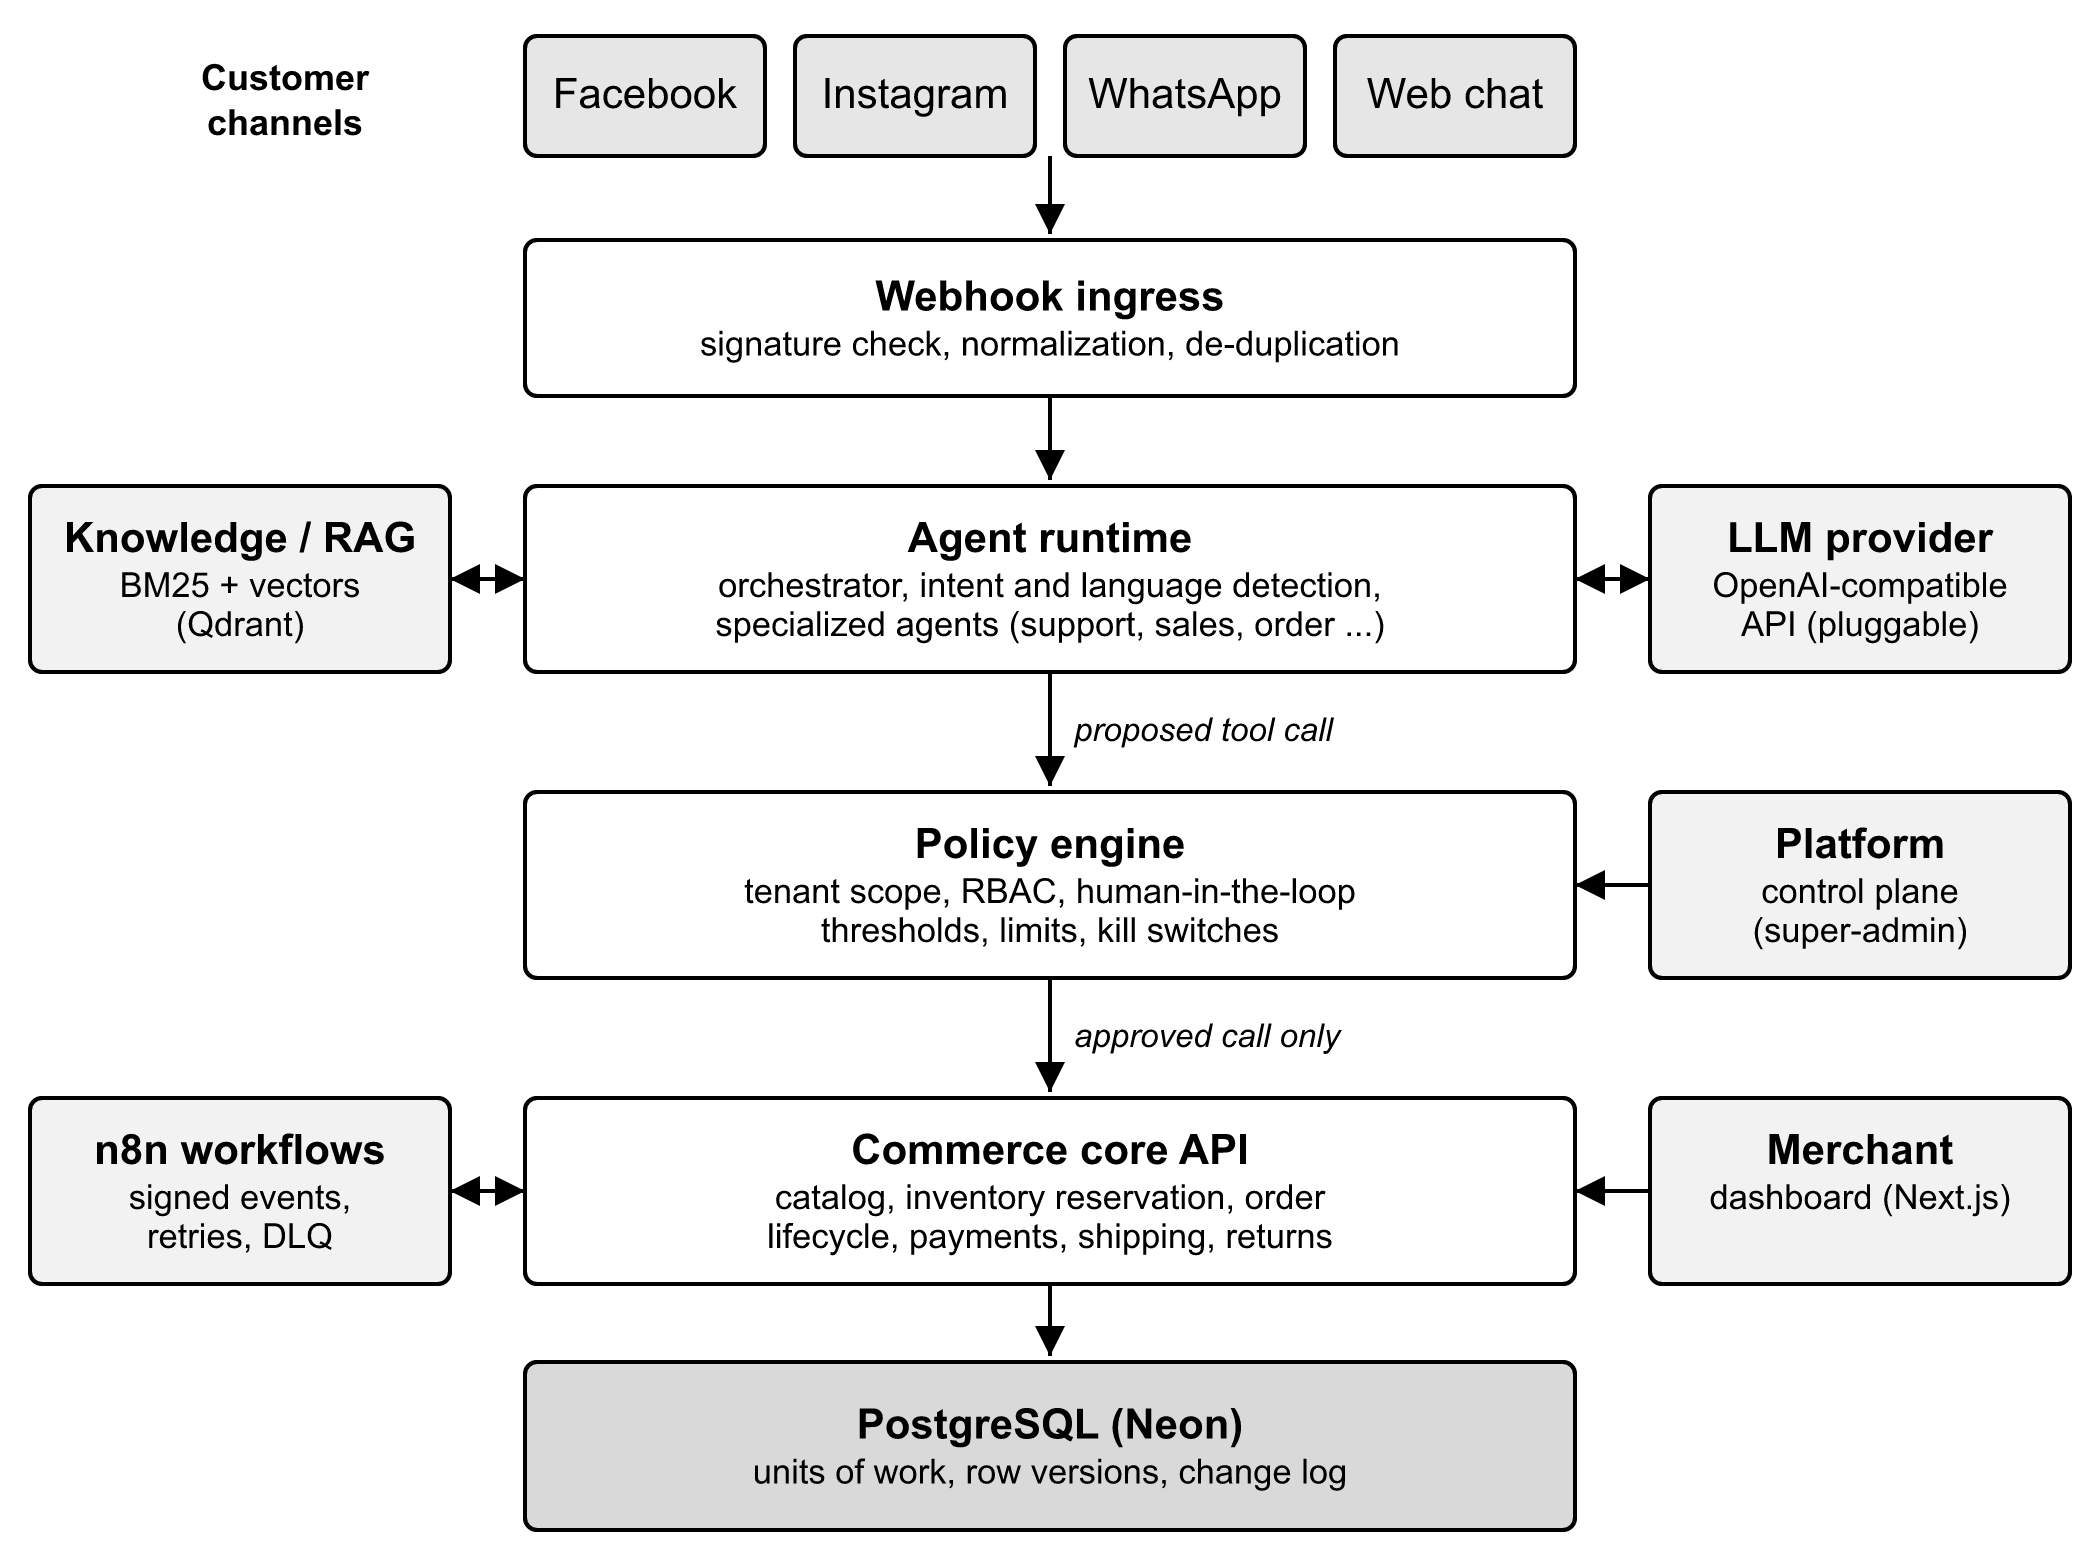
\includegraphics[width=\columnwidth]{fig-architecture.png}
\caption{Layered architecture of CommerceOS. Agents may only propose tool calls; the policy engine decides which reach the commerce core.}
\label{fig:arch}
\end{figure}

\subsection{Architecture Overview}
Fig. 1 shows the architecture. The application is written in TypeScript (strict mode) on Next.js with React; a versioned REST API (/api/v1) exposes 26 domain modules. PostgreSQL on Neon is the system of record, Qdrant stores vectors, n8n runs asynchronous workflows, and the LLM is any OpenAI-compatible provider selected by configuration (e.g., OpenAI, OpenRouter, Groq, DeepSeek, or a local Ollama or vLLM server).

\subsection{Deterministic Commerce Core}
A single service owns order status and enforces the lifecycle Pending, Confirmed, Processing, Shipped, Delivered, with Cancelled and Returned as exits. Stock is reserved when an order is created and released when the reservation expires. Delivery fees come from tenant settings, never from prompts. A payment screenshot alone never marks an order paid; verification rules must pass first.

\subsection{Policy-Governed Agents}
Each agent has an allowlist of tools in a central registry (Table I). When an agent proposes a call, the policy engine checks tenant scope, the caller's permission, platform kill switches and risk thresholds; high-risk actions go to a human approval queue. The LLM never writes to storage, and any price, stock or order value in a reply is taken from a tool result in the same turn. This is the property tested by RQ1.

\begin{table}[!t]
\renewcommand{\arraystretch}{1.2}
\caption{Example Agent Roles and Tool Boundaries (Design)}
\label{tab:1}
\centering\footnotesize
\begin{tabular}{|p{0.19\columnwidth}|p{0.36\columnwidth}|p{0.31\columnwidth}|}
\hline
\textbf{Agent} & \textbf{Allowed tools (examples)} & \textbf{Forbidden or approval-gated} \\
\hline
Support & knowledge search, order lookup, policy lookup & order cancel, refund \\
\hline
Sales & product search, stock check, lead create & arbitrary discounts, direct orders \\
\hline
Order & order status, propose update & hard delete, refund execute \\
\hline
Payment & payment status, transaction lookup & manual mark-as-verified \\
\hline
Marketing & segments, campaign draft & mass send (human approval) \\
\hline
\end{tabular}
\end{table}

\subsection{Knowledge Retrieval}
Merchant documents are chunked and indexed twice: in an in-process BM25 index and as dense vectors in Qdrant, filtered by tenant. The two ranked lists are fused with RRF (k = 60). When retrieval confidence is below a threshold the agent hands the conversation to a human instead of answering.

\subsection{Security Architecture}
The tenant is taken only from the authenticated session, never from request data, and every lookup by identifier also filters by tenant. Every mutating API handler checks a permission against ten workspace roles plus a scoped service role. Tokens are JWTs with an issuer and a per-purpose audience; passwords use bcrypt; platform operators use TOTP MFA with step-up for sensitive actions. Courier and payment webhooks carry an HMAC over a timestamp and the raw body, checked within a 300 s window with duplicate suppression. All outbound HTTP calls pass through one client that blocks server-side request forgery (SSRF). Support staff can view a tenant only through read-only, audited sessions.

\subsection{Persistence and Honest Integrations}
Each write request is one unit of work, committed to PostgreSQL with row-version checks and a change log before the response is sent, so several application servers can share one database. Integrations that are not yet connected report NOT\_SENT or SIMULATED and never report success; no dashboard shows fabricated metrics.


\section{Methodology}
\subsection{Development Process}
Development is iterative and phase-gated. Requirements follow ISO/IEC/IEEE 29148~\cite{iso29148}; design decisions are recorded as architecture decision records in the spirit of IEEE 1016~\cite{ieee1016}. A task is done only when the type-checker reports zero errors, all test suites pass, the wiring from user interface to route to service to store has been traced, and the status registry is updated.

\subsection{Truthful Status Registry}
Every capability is labelled LIVE, PARTIAL, SIMULATED, STATIC, BROKEN or TARGET in a single registry, and documentation may not claim a capability exists unless the registry marks it LIVE. This keeps the thesis report, the demo and the code consistent.

\subsection{Security-First Remediation}
An independent audit of the prototype on 27 September 2026 identified critical and high-severity findings (for example authentication shortcuts, unsigned webhooks and missing permission checks). They were fixed in ordered phases (containment, access control, read-path integrity, truthful data, and migration to PostgreSQL), each merged and tagged only after its regression tests passed.

\subsection{Testing}
Tests are custom TypeScript suites: security regression tests for each audit finding, an RBAC matrix over the mutating handlers, tenant-isolation negative tests, a read-only sweep proving that no GET route writes, a PostgreSQL round-trip suite on an embedded database, an exploit-replay script against a running server, and an offline evaluation gate over a golden dataset for the agents.


\section{Current State of the Prototype}
Table II summarizes the prototype as of 29 September 2026. The system is not production-ready and is not exposed to any public network.

\begin{table}[!t]
\renewcommand{\arraystretch}{1.2}
\caption{Prototype Metrics (29 September 2026)}
\label{tab:2}
\centering\footnotesize
\begin{tabular}{|p{0.53\columnwidth}|p{0.33\columnwidth}|}
\hline
\textbf{Item} & \textbf{Value} \\
\hline
TypeScript source files / lines & 659 / approx. 108,000 \\
\hline
API route files / domain modules & 251 / 26 \\
\hline
Automated test suites / tests passing & 27 / 872 \\
\hline
Type-check errors; production build & 0; passes \\
\hline
Workspace roles (+ service role) & 10 (+1) \\
\hline
Exported n8n workflows & 9 \\
\hline
System of record & PostgreSQL (Neon) \\
\hline
\end{tabular}
\end{table}

Working today: authentication with MFA and revocable sessions, tenant-scoped RBAC, signed webhooks, the order lifecycle with stock reservation, the merchant dashboard on real data, and PostgreSQL persistence shared by several servers. Not yet built: the live Messenger, Instagram and WhatsApp send paths, courier booking and bKash/Nagad verification against real provider APIs; these currently report NOT\_SENT. Write requests take about 2 to 4 s when the server is far from the database region, which must be fixed by co-locating them. The audit's capability census found 41 of 122 capabilities fully working at the time, a baseline this project will raise and report honestly.


\section{Evaluation Plan}
Table III lists the measures for each research question. Targets are acceptance thresholds for the project, not claimed results.

\begin{table}[!t]
\renewcommand{\arraystretch}{1.2}
\caption{Evaluation Measures and Targets}
\label{tab:3}
\centering\footnotesize
\begin{tabular}{|p{0.10\columnwidth}|p{0.45\columnwidth}|p{0.31\columnwidth}|}
\hline
\textbf{RQ} & \textbf{Measure and method} & \textbf{Target} \\
\hline
RQ1 & Critical-value fidelity: share of price, stock, payment and order values in agent replies that match a tool result of the same turn, over at least 500 scripted conversations including prompt-injection attempts & 100\% \\
\hline
RQ1 & Automation rate: routine inquiries resolved without a human & Report; aim at least 60\% \\
\hline
RQ2 & Recall@5 and MRR@10 of BM25, dense and hybrid retrieval on at least 300 labelled queries in three language styles; paired significance test~\cite{smucker} & Hybrid better, p $<$ 0.05 \\
\hline
RQ3 & Cross-tenant and privilege-escalation attempts blocked in the RBAC matrix and exploit replay; ASVS Level 2 items covered & 100\% blocked \\
\hline
Perf. & p95 latency with server and database co-located: API reads, writes, first agent reply & $<$ 0.5 s, $<$ 1 s, $<$ 5 s \\
\hline
RQ4 & RTO rate before and after automated COD confirmation, 2 to 3 merchants over 4 to 8 weeks & Descriptive only \\
\hline
\end{tabular}
\end{table}

Evaluation data will combine synthetic conversations with anonymized, consented merchant data. Native speakers will label intents and relevance, and inter-annotator agreement will be reported with Cohen's kappa~\cite{cohen}. Because the pilot is small, RQ4 results will be reported descriptively without claims of generality.


\section{Work Plan and Resources}
\subsection{Timeline}
The project spans about 28 weeks over two semesters, starting October 2026 (Table IV).

\begin{table}[!t]
\renewcommand{\arraystretch}{1.2}
\caption{Work Plan}
\label{tab:4}
\centering\footnotesize
\begin{tabular}{|p{0.15\columnwidth}|p{0.71\columnwidth}|}
\hline
\textbf{Weeks} & \textbf{Activity and milestone} \\
\hline
1--3 & Literature review; interviews with 3 to 5 merchants; software requirements specification (M1) \\
\hline
4--7 & Messenger, Instagram and WhatsApp integration in sandbox \\
\hline
8--10 & Courier and bKash sandbox integration; co-located deployment (M2) \\
\hline
11--14 & Multilingual dataset and agent evaluation harness; RQ1 experiments \\
\hline
15--17 & Retrieval experiments (RQ2); interim report (M3) \\
\hline
18--20 & Security evaluation (RQ3) and performance tuning \\
\hline
21--25 & Merchant pilot (RQ4), subject to ethics approval (M4) \\
\hline
26--28 & Analysis, final report, demonstration and defense (M5) \\
\hline
\end{tabular}
\end{table}

\subsection{Resources}
Development uses a personal computer and open-source tools. Running costs are managed cloud PostgreSQL, application hosting and pay-per-use LLM calls; provider sandboxes are free. Using free tiers and a capped LLM budget, the estimated total is below US\$500 for the whole project. This estimate will be confirmed against current provider pricing before work begins.


\section{Risks, Ethics and Limitations}
\subsection{Risks and Mitigation}
\begin{itemize}
\item Provider access: Meta business verification or courier and payment API approval may be slow. Mitigation: start in week 1 and develop against sandboxes and recorded fixtures.
\item LLM cost and latency: mitigated by model routing (smaller models for simple intents), caching and a hard budget.
\item Scarce Banglish data: mitigated by building and releasing a labelled dataset as part of the project.
\item Pilot recruitment: if no merchant can take part, RQ4 is dropped and RQ1 to RQ3 still stand on offline evaluation.
\item Security regressions: no network exposure until the regression suites and exploit replay pass.
\end{itemize}

\subsection{Ethics and Privacy}
Merchant and customer data contain personal information (names, phone numbers, addresses). The project will obtain university ethics approval and written merchant consent before the pilot, minimize and anonymize data used for evaluation, follow applicable Bangladeshi data-protection requirements, tell customers when they are talking to an AI assistant, and always offer escalation to a human.


\section{Expected Outcomes}
\begin{itemize}
\item A documented reference architecture for policy-governed agentic commerce.
\item A working prototype with at least one live messaging channel, courier and payment sandbox integration.
\item A labelled Bangla, English and Banglish commerce query dataset and an evaluation harness.
\item Empirical answers to RQ1 to RQ3, and to RQ4 if the pilot runs.
\item A final report, a demonstration, and a paper submitted to a peer-reviewed conference if the results support it.
\end{itemize}


\section{Conclusion}
CommerceOS addresses a real and underserved setting: conversational, COD-heavy commerce in Bangladesh. Its central idea is that AI agents may converse and propose actions, but only a deterministic, policy-guarded commerce core may state or change business facts. A substantial, audited prototype makes the project feasible within two semesters, and the research questions give it measurable outcomes beyond the software itself.


\begin{thebibliography}{00}
\bibitem{yao} S. Yao \textit{et al.}, ``ReAct: Synergizing reasoning and acting in language models,'' in \textit{Proc. Int. Conf. Learning Representations (ICLR)}, 2023.
\bibitem{schick} T. Schick \textit{et al.}, ``Toolformer: Language models can teach themselves to use tools,'' in \textit{Proc. Advances in Neural Information Processing Systems (NeurIPS)}, vol. 36, 2023.
\bibitem{wang} L. Wang \textit{et al.}, ``A survey on large language model based autonomous agents,'' \textit{Frontiers of Computer Science}, vol. 18, no. 6, Art. no. 186345, 2024.
\bibitem{ji} Z. Ji \textit{et al.}, ``Survey of hallucination in natural language generation,'' \textit{ACM Computing Surveys}, vol. 55, no. 12, pp. 1--38, 2023.
\bibitem{greshake} K. Greshake, S. Abdelnabi, S. Mishra, C. Endres, T. Holz, and M. Fritz, ``Not what you've signed up for: Compromising real-world LLM-integrated applications with indirect prompt injection,'' in \textit{Proc. 16th ACM Workshop on Artificial Intelligence and Security (AISec)}, 2023, pp. 79--90.
\bibitem{owaspllm} OWASP Foundation, ``OWASP Top 10 for Large Language Model Applications,'' 2025. [Online]. Available: \url{https://genai.owasp.org/}
\bibitem{chong} F. Chong and G. Carraro, ``Architecture strategies for catching the long tail,'' Microsoft Corp., Redmond, WA, USA, Tech. Rep., Apr. 2006.
\bibitem{guo} C. J. Guo, W. Sun, Y. Huang, Z. H. Wang, and B. Gao, ``A framework for native multi-tenancy application development and management,'' in \textit{Proc. 9th IEEE Int. Conf. E-Commerce Technology and 4th IEEE Int. Conf. Enterprise Computing, E-Commerce and E-Services (CEC/EEE)}, 2007, pp. 551--558.
\bibitem{lewis} P. Lewis \textit{et al.}, ``Retrieval-augmented generation for knowledge-intensive NLP tasks,'' in \textit{Proc. Advances in Neural Information Processing Systems (NeurIPS)}, vol. 33, 2020, pp. 9459--9474.
\bibitem{gao} Y. Gao \textit{et al.}, ``Retrieval-augmented generation for large language models: A survey,'' arXiv:2312.10997, 2023.
\bibitem{robertson} S. Robertson and H. Zaragoza, ``The probabilistic relevance framework: BM25 and beyond,'' \textit{Foundations and Trends in Information Retrieval}, vol. 3, no. 4, pp. 333--389, 2009.
\bibitem{cormack} G. V. Cormack, C. L. A. Clarke, and S. Buettcher, ``Reciprocal rank fusion outperforms Condorcet and individual rank learning methods,'' in \textit{Proc. 32nd Int. ACM SIGIR Conf. Research and Development in Information Retrieval}, 2009, pp. 758--759.
\bibitem{nogueira} R. Nogueira and K. Cho, ``Passage re-ranking with BERT,'' arXiv:1901.04085, 2019.
\bibitem{bhattacharjee} A. Bhattacharjee \textit{et al.}, ``BanglaBERT: Language model pretraining and benchmarks for low-resource language understanding evaluation in Bangla,'' in \textit{Findings of the Association for Computational Linguistics: NAACL 2022}, 2022, pp. 1318--1327.
\bibitem{asvs} OWASP Foundation, ``Application Security Verification Standard 4.0.3,'' 2021. [Online]. Available: \url{https://owasp.org/www-project-application-security-verification-standard/}
\bibitem{sandhu} R. S. Sandhu, E. J. Coyne, H. L. Feinstein, and C. E. Youman, ``Role-based access control models,'' \textit{Computer}, vol. 29, no. 2, pp. 38--47, Feb. 1996.
\bibitem{jwt} M. Jones, J. Bradley, and N. Sakimura, ``JSON Web Token (JWT),'' IETF RFC 7519, May 2015.
\bibitem{totp} D. M'Raihi, S. Machani, M. Pei, and J. Rydell, ``TOTP: Time-based one-time password algorithm,'' IETF RFC 6238, May 2011.
\bibitem{hmac} H. Krawczyk, M. Bellare, and R. Canetti, ``HMAC: Keyed-hashing for message authentication,'' IETF RFC 2104, Feb. 1997.
\bibitem{fowler} M. Fowler, \textit{Patterns of Enterprise Application Architecture}. Boston, MA, USA: Addison-Wesley, 2002.
\bibitem{helland} P. Helland, ``Life beyond distributed transactions: An apostate's opinion,'' in \textit{Proc. 3rd Biennial Conf. Innovative Data Systems Research (CIDR)}, 2007, pp. 132--141.
\bibitem{kleppmann} M. Kleppmann, \textit{Designing Data-Intensive Applications}. Sebastopol, CA, USA: O'Reilly Media, 2017.
\bibitem{garcia} H. Garcia-Molina and K. Salem, ``Sagas,'' in \textit{Proc. ACM SIGMOD Int. Conf. Management of Data}, 1987, pp. 249--259.
\bibitem{iso29148} \textit{Systems and Software Engineering---Life Cycle Processes---Requirements Engineering}, ISO/IEC/IEEE 29148:2018, 2018.
\bibitem{ieee1016} \textit{IEEE Standard for Information Technology---Systems Design---Software Design Descriptions}, IEEE Std 1016-2009, 2009.
\bibitem{smucker} M. D. Smucker, J. Allan, and B. Carterette, ``A comparison of statistical significance tests for information retrieval evaluation,'' in \textit{Proc. 16th ACM Conf. Information and Knowledge Management (CIKM)}, 2007, pp. 623--632.
\bibitem{cohen} J. Cohen, ``A coefficient of agreement for nominal scales,'' \textit{Educational and Psychological Measurement}, vol. 20, no. 1, pp. 37--46, 1960.
\end{thebibliography}

\end{document}
